\lhead{\textbf{Basic Algorithms, Fall 2024 \\ CSCI-UA.0310-001}}
\chead{\Large{\textbf{Homework 11}}}
\def\lc{\left\lceil}   
\def\rc{\right\rceil}
\newtheorem{claim}{Claim}
\newtheorem{property}{Property}
\rhead{\textbf{Instructor: Rotem Oshman \\ Name: Ishan Pranav}}
\runningheadrule
\firstpageheadrule
\cfoot{}
\stepcounter{subsection}
\section*{References}
Collaborated with Crystal Huang.
\subsection{Prim and Kruskal}
\begin{figure}[h]
    \centering
    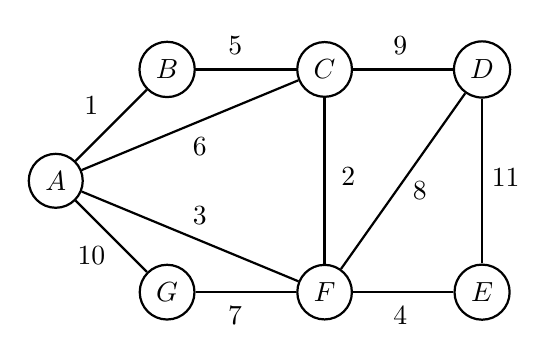
\begin{tikzpicture}[node distance={20mm}, thick,main/.style={circle, thick,draw,font=\sffamily\bfseries}, ar/.style={-{Stealth[scale=1.2]}}]
      \node[main] (1) {$A$}; 
      \node[main] (2) [above right of=1]{$B$};
      \node[main] (3) [right of=2]{$C$};
      \node[main] (4) [right of=3]{$D$};
      \node[main] (5) [below right of=1]{$G$};
      \node[main] (6) [right of=5]{$F$};
      \node[main] (7) [right of=6]{$E$};
      
      \draw (1) -- (2) node [at start, xshift=0.2cm, yshift=0.7cm]{$1$};
      \draw (1) -- (3) node [at start, xshift=1.5cm, yshift=0.3cm]{$6$};
      \draw (1) -- (5) node [at start, xshift=0.2cm, yshift=-0.7cm]{$10$};
      \draw (1) -- (6) node [at start, xshift=1.5cm, yshift=-0.3cm]{$3$};
      \draw (2) -- (3) node [at start, xshift=0.5cm, yshift=0.3cm]{$5$};
      \draw (3) -- (4) node [at start, xshift=0.6cm, yshift=0.3cm]{$9$};
      \draw (3) -- (6) node [at start, xshift=0.3cm, yshift=-1.0cm]{$2$};
      \draw (4) -- (7) node [at start, xshift=0.3cm, yshift=-1.0cm]{$11$};
      \draw (5) -- (6) node [at start, xshift=0.5cm, yshift=-0.3cm]{$7$};
      \draw (6) -- (7) node [at start, xshift=0.6cm, yshift=-0.3cm]{$4$};
      \draw (6) -- (4) node [at start, xshift=1.0cm, yshift=1.0cm]{$8$};
    \end{tikzpicture}
    \caption{\textbf{Undirected graph $\mathbf{G}$.}}
    \label{fig:mst}
\end{figure}

Consider the undirected weighted graph $G = (V, E)$ in Figure~\ref{fig:mst} above.
\begin{enumerate}
    \item  Illustrate a run of Kruskal's algorithm on this graph. State at each step which edge is added to the tree. We have filled the first step in for you. Here, we only want the edge added to the tree and not every edge that is considered. 
    
    \begin{center}
    \begin{tabular}{c|c|c|c|c|c|c|c}
         \textbf{Step} & 1 & 2 & 3 & 4 & 5 & 6\\
         \hline
         \textbf{Edge Added} & $AB$ &   &   &   &   & \\
    \end{tabular}
    \end{center}
\begin{solution}   INSERT YOUR SOLUTION HERE   \end{solution}
    \item Illustrate a run of Prim's algorithm on this graph starting from vertex $A$. State at each step which edge is added to the tree. We have filled the first step in for you. Here, we only want the edge added to the tree and not every edge that is considered. 
    
    \begin{center}
    \begin{tabular}{c|c|c|c|c|c|c|c}
         \textbf{Step} & 1 & 2 & 3 & 4 & 5 & 6\\
         \hline
         \textbf{Edge Added} & $AB$ &   &   &   &   &  \\
    \end{tabular}
    \end{center}
\begin{solution}   INSERT YOUR SOLUTION HERE   \end{solution}
\end{enumerate}


\subsection{Minimal spanning tree}
Prove or disprove the following statements. If true, give a short explanation. If false, give a counterexample.

\begin{enumerate}
\item Let $G = (V, E)$ be a connected, undirected graph with a distinct cost $c(e)$ on every edge $e$. Suppose $e^*$ is the cheapest edge in $G$; that is, $c(e^*) < c(e)$ for every edge $e \neq e^*$. Then there is a minimum spanning tree $T$ of $G$ that contains the edge $e^*$.
\begin{solution}

\textbf{Definition I. }Let $G=(V,E)$ be a connected, undirected graph with a distinct cost $c(e)$ for every edge $e\in E$.

\textbf{Definition II. }Let $e^*\in E$ be the cheapest edge in $G$; that is, we have $c(e^*)<c(e)$ for all $e\in E$ where $e\neq e^*$.

\textbf{Lemma I. }\textit{Claim. }Let $T=(V,E_T)$ be a spanning tree of $G$ where $e^*\notin T$. We can construct a spanning tree of $G$ whose total cost is less than that of $T$.

Since $T$ is a spanning tree of $G$, there exists a path $(u,\dots,x,y,\dots,v)$ in $T$ containing an edge $e'=\{x,y\}$ for $x,y\in V$. Of course, $e'\neq e^*$ since $T$ does not contain $e^*$.

We can add edge $e^*$ to $T$ to construct $T'=(V,E_T\cup\{e^*\})$, an induced subgraph of $G$. Now there exists a cycle $(u,\dots,x,y,\dots,v,u)$ in $T'$ that contains $e'$. Note that $T'$ is connected because $T$ is a tree, and thus connected.

We can construct $T''=(V,(E_T\cup\{e^*\})\setminus\{e'\})$, an induced subgraph of $G$ derived by replacing $e^*$ with $e'$ in $T$; that is, by removing $e'$ from $T'$.

After severing the edge $e'=\{x,y\}$, paths $(x,\dots,u)$ and $(v,\dots,y)$ still do exist in $T''$. Since edge $e=\{u,v\}$ does exist in $T''$, there exists a path $(x,\dots,u,v,\dots,y)$ in $T''$. All other vertices in $T''$ are connected because $T'$ is connected. So $T''$ is connected. 

Without $e'=\{x,y\}$, the cycle $(u,\dots,x,y,\dots,v,u)$ does not exist in $T''$. By construction, this is the only cycle in $T''$ since $T$ is a tree, and thus, acyclic. Thus, $T''$ is acyclic.

By construction of $T''$, the total cost of all edges in $T''$ is the total cost of all edges in $T$, minus the cost of $e'$, plus the cost of $e^*$. Since $c(e^*)$ is the cheapest edge in $G$, and $e'\in G$, we know $c(e^*)<c(e')$. Therefore, the total cost of all edges in $T''$ is less than that of all edges in $T$.

Since $T''$ is a connected, acyclic, induced subgraph of $G$ containing all vertices in $G$, we know that $T''$ is a spanning tree. $T''$ is a spanning tree of $G$ with a smaller total cost than $T$---what was to be constructed.

\textbf{Proposition I. }\textit{Claim. }There exists a minimum spanning tree of $G$ that contains $e^*$.

\textit{Proof. }Assume, for the sake of contradiction, that there exists no minimum spanning tree of $G$ that contains edge $e^*=\{u,v\}$ for $u,v\in V$. Let $T=(V,E_T)$ be a minimum spanning tree of $G$. It follows from our hypothesis that $e^*\notin E_T$.

From Lemma I, since $T$ is a spanning tree of $G$ that does not contain its cheapest edge $e^*$, we can construct a spanning tree of $G$ whose total cost is less than that of $T$.

This is absurd: It contradicts the hypothesis that $T$ is a \textit{minimum} spanning tree of $G$. Ergo, the hypothesis is false: There does exist a minimum spanning tree of $G$ containing $e^*.~\square$
\end{solution}
\newpage
\item In the above setting, every MST of $G$ contains the edge $e^*$.
\begin{solution}
\textbf{Proposition II. }\textit{Claim. }Every minimum spanning tree of $G$ contains $e^*$.

\textit{Proof. }Assume, for the sake of contradiction, that there exists some minimum spanning tree $T=(V,E_T)$ of $G$ where $e^*\notin E_T$.

From Lemma I, since $T$ is a spanning tree of $G$ that does not contain its cheapest edge $e^*$, we can construct a spanning tree of $G$ whose total cost is less than that of $T$.

This is absurd: It contradicts the hypothesis that $T$ is a \textit{minimum} spanning tree of $G$. Ergo, the hypothesis is false: Every minimum spanning tree of $G$ does contain $e^*.~\square$
\end{solution}
\newpage
\end{enumerate}
\subsection{Faster minimal spanning tree}
\begin{enumerate}
    \item Assume that all edge weights of the given undirected graph $G = (V, E)$ are promised to be $1$. Design the fastest algorithm you can to compute the minimum spanning tree (MST) of $G$. Argue the correctness of the algorithm and state its run-time. 
    
    \hint{It should be more efficient than the $O(|E| \log |V|)$ run-time of Prim and Kruskal.}
\begin{solution}

\textbf{Algorithm 1. }{\sc SpanningTree}($G$) with undirected graph $G=(V,E)$, returns a minimum spanning tree of $G$:

Let $T=(V,E_T)$ with $E_T\leftarrow\emptyset$.

If $V=\emptyset$, then return $T$.

Let $s\leftarrow v\in V$, choosing $s$ arbitrarily.

Perform {\sc DepthFirstSearch}($s,G$); here {\sc DepthFirstSearch} is the well-known depth-first-search algorithm that visits each vertex in a graph once beginning from a source $s\in V$ and assigning $u.\mathsf{parent}$ to some vertex $v\in V$ for each $u\in V\setminus\{s\}$. Note {\sc DepthFirstSearch} has running time $O(|V|+|E|)$.

For $v\in V\setminus\{s\}$, assign $E_T\leftarrow E_T\cup\{\{v.\mathsf{parent},v\}\}$, via adjacency list.

Return $T$.

\textbf{Proposition 1. }\textit{Claim. }{\sc SpanningTree}($G$) is correct.

\textit{Proof. }

\textbf{Proposition 2. }\textit{Claim. }{\sc SpanningTree}($G$) has running time $O(|V|+|E|)$.

\textit{Proof. }First, Algorithm 1 invokes {\sc DepthFirstSearch} with running time $O(|V|+|E|)$.

Then, for each of the $|V|-1$ vertices in $V\setminus\{s\}$, it inserts an edge into $T$ via adjacency list, an $O(1)$ operation. Thus, the running time of the loop is $O(|V|)$.

Finally, Algorithm 1 returns the resulting tree, an $O(1)$ operation.

Thus, the running time of {\sc SpanningTree}($G$) is $O(|V|+|E|)+O(|V|)=O(|V|+|E|).~\square$
\end{solution}
    \item Suppose instead that all edge weights are 1 \emph{except} for a single edge $e_0 = (u_0, v_0)$ whose weight is $w_0$ (note, $w_0$ might be either larger or smaller than 1). Show how to modify your solution in part 1 to compute the MST of $G$. What is the running time of your algorithm and how does it compare to the runtime you obtained in part 1 (or standard Prim)?
\begin{solution}   INSERT YOUR SOLUTION HERE   \end{solution}
\end{enumerate}